\chapter{From Bloom filters to Bloomaps}

During points-to analysis the datastructure is almost as important as the
algorithm used. In the case of GCC, the structure chosen is a hybrid of bitmap
and a linked list. This works fine for small and dense data, but not so well
with large data. Converting to a better data structure is relatively easy task, but what data
structures are available? We will start by examining the needs of a typical
Andersen-style algorithm and comparing theoretical complexities of various well
known data structures. In the rest of this chapter we will describe a new
enhancement of bloom filters called Bloomaps, tailored specifically for the use
in points-to analysis.

\section{Requirements}

As a basic data structure for PTA, we need a data structure holding sets of
integers that is compact and has the following operations.

\begin{itemize}
	\item {\tt INSERT(set, element)} -- inserts {\tt element} into {\tt set} and returns if
		the structure has been changed by the insertion.
	\item {\tt QUERY(set, element)} -- checks if {\tt element} is part of {\tt set}.
	\item {\tt INTERSECT\_EMTPY(set1, set2)} -- checks if intersection of {\tt
		set1} and {\tt set2} is empty.
	\item {\tt ENUMERATE(set)} -- lists all elements in a {\tt set}.
	\item {\tt UNION(set1, set2)} -- merge {\tt set2} into {\tt set1}.
\end{itemize}

The algorithm uses the following operations in the following way:

\begin{itemize}
	\item Initialization: {\tt INSERT} for every set.
	\item Propagation: {\tt UNION} for every simple constraint, {\tt ENUMERATE} and
		{\tt UNION} for dereferences.
	\item Oracle queries: {\tt QUERY} for set membership, {\tt INTERSECT\_EMPTY}
		for set disjointness
\end{itemize}

In other words, the basic operations can be slower, {\tt UNION} and {\tt
INTERSECT\_EMPTY} has to be fast. There are a few other considerations:

\begin{itemize}
	\item The {\tt UNION} will be called on the same pairs over and over again,
		the difference will usually be in just a few elements.
	\item The average number of stored elements will be small, and the data sparse.
	\item Some sets may grow very large, containing almost every element possible.
	\item Low memory overhead is required, as the number of sets is in the order
		of number of elements inserted.
\end{itemize}

A simple bitmap is a straightforward solution, but the sparseness make it
unviable. Many tree-like structures will have problems with the intersections
and union as all the elements have to examined and deduplicated. Structures
requiring pointers, storing element values or hashes do have large overhead.

A natural choice of the datastructure is a bloom filter. It is compact, has a
fast union and allows us to choose how much memory to invest and sacrifice the
precision if we don't have enough. Unfortunately, its performance in {\tt
INTERSECT} is rather suboptimal, and even worse, completely lacks the {\tt
ENUMERATE} operation.


\section{Bloom filters}

A bloom filter is a classical probabilistic data structure, invented by Burton
Howard Bloom \cite{Bloom1970}. The goal is to provide a data structure
that has some nonzero probability of {\it false-positive}, but zero probability
of {\it false-negative}. This is accomplished by taking a bit field of $m$ bits,
$k$ hash functions, and hashing every element into $k$ different bits, writing
$1$ on insertion, and checking if every position contains $1$ on query.

The Bloom filter has immediate applications in some areas, for example caching:
it is a good idea to ask a filter if an element is in the cache. If the answer is
no, we need to get it elsewhere. If the answer is yes, we can look into the
cache, and in the worst case it is not there (an ocurrence false-positive).

Here is a short list of properties (provided the hashes can be computed in
constant time, which is often possible).:

\begin{itemize}
	\item {\tt QUERY} in $\O(1)$ time.
	\item {\tt INSERT} in $\O(1)$ time.
	\item {\tt DELETE, ENUMERATE, RESIZE} not supported\footnote{Though there
		are variations that support these oprations, only {\tt RESIZE} is usually
		possible without drastic changes to the structure.}.
	\item {\tt UNION} in $\O(m)$ time (bitwise OR).
	\item {\tt BITWISE\_INTERSECTION} in $\O(m)$ time.
\end{itemize}

Unlike in simple bitmaps, bitwise intersection of bloom filters is not equal to
set intersection.  Let's denote $BF(A)$ as a bloom filter created from empty
filter by inserting elements from $A$ one by one. Then:

For $A,B$ it does not hold that $BF(A \cap B) = BF(A) \cap
BF(B)$. Unfortunately, even the inequality $BF(A \cap B) \subseteq BF(A) \cap
BF(B)$ holds, it is nowhere near the equality. Most imporantly, we would like to
check for emptyness of intersection, which is hard to achieve.

\section{Bloom filter intersection}

Although a bloom filter intersection easily computed with bitwise {\tt AND},
it is rarely accurate. The basic properties are already understood:

As proven in \cite{bose2008false}, the probability that $BF(A\cap B) =
BF(A) \cap BF(B)$ is:
\begin{align}
p = (1-1/m)^{k^2\cdot |A-A\cap B| \cdot |B - A\cap B|}
\end{align}

For set emptyness, we can further simplify the formula by separating two cases:
$|A \cap B| > 0$ and $|A \cap B| = 0$. The second equality is interesting, as
we would like to test for empty sets.

Assuming that $|A\cap B| = 0$, let us compute the probability that $BF(A) \cap
BF(B)$ is also empty.
\begin{align}
	p_{empty} = (1-1/m)^{k^2 \cdot |A| \cdot |B|}
\end{align}

Furthermore, if we use partitioned Bloom filters, Jeffrey and Steffan
[REF:Jeffrey11] showed a slightly improved bound:
\begin{align}
	p_{empty} = \left(1 - \left( 1 - {k \over m}\right)^{|A|\cdot |B|}\right)^k
\end{align}

This is due to the fact that it is enough to have one empty partition to consider
the filter empty, as every query would result in false in the empty partition.

However, in the same article they proved that pure Bloom filter intersection is more
memory-consuming than more conventional queue-of-queries. In the next section,
a hybrid solution is provided that can be used with both of these approaches,
based on the time requirements.

\section{Bloom filter enumeration}

It's immediately clear that vanilla Bloom filter cannot provide list of it's
possible elements, as for example the simplest filter holding $1$ elements and
answering with false-positive probability $0.5$ would have to enumerate half the
universe $U$, which may as well be impossible for $U=\N$.

Besides the trivial queue-of-queries, there has been one attempt at constructing
Bloom filter-like structure, that can list it's items, the Invertible Bloom
Lookup Tables (IBLT), by Michael T. Goodrich \cite{goodrich:2011}. The problem of IBLT is
that they have non-zero probability of being unable to produce a complete list
of entries, and do not provide the advantages of classic Bloom filters, as a
fast intersection and membership queries. This said, we will not attempt to use
them, although they are an interesting structure for future work and may find
its use in other optimizers.

Let us review in short the available methods:

\paragraph{Enumerate entire universe.} This is possible for small and dense
universe, and appropriately sized filter. We don't have to keep extra data, but
queries need to ask for every element in a universe. Even for almost empty
filter, this approach takes $\O(|U|)$ time.

\paragraph{Keep a Queue-of-queries for each filter.} Perhaps the most sensible
way, if there are either few filters, or only a few elements in each filter.
This approach may fast insertion and query, though complexity of the
Queue-of-queries structure needs to be taken into account and either we need to
sacrifice more memory to store unsorted queue, or time to use a better data
structure for the queue.

Neither of these methods are good for our use, as our universe can be large
(millions of lines of code), and the number of filters is about the same size as
the universe. We introduce a new approach, a compromise between the two above.

\paragraph{Keep a single Queue-of-queries for all filteris.}

Assuming our universe is all 32 bit integers, we can store a bit array of every
item ever inserted under 512 MB. This allows the universe to be relatively
sparse (we can skip unused elements). Also the operations only need to perform
$\O(1)$ extra work to write a new bit, which is reasonable.

\section{Bloomaps and Families}

\paragraph{Definition.} Bloomap Family with parameters $(m, k, s)$ is a
datastructure that maintains a list of Bloomaps of the same parameters, and
indexed representation of used parts of the universe in union of all it's
Bloomaps, capable of enumeration.

\paragraph{Definition.} Bloomap is an enhanced Bloom filter, belonging to a single
family, capable of executing {\tt INSERT} and {\tt QUERY} itself, and {\tt
ENUMERATE}, {\tt UNION} and {\tt INTERSECT} within it's family.

A bloomap with parameters $(m, k, s)$ is constructed from a partitioned Bloom
filter with the addition of a {\it side index} containing $s$ bits. The side
index is used as another partition in the bloomfilter, however with simpler hash
function that is easily inverted (for example a simple {\tt SHIFT} and {\tt
AND} with a mask).

Furthermore, the Bloomaps and their families need to fulfill these conditions:

\begin{itemize}
	\item When a new item is inserted into a Bloomap, it is also inserted into
		the family.
	\item A Family has to enumerate all items inserted into it's Boomaps for any
		given hash.
\end{itemize}

\begin{figure}[h!]
\begin{tcolorbox}
	\begin{lstlisting}[language=c++,tabsize=2]
struct Bloomap {
    BloomapFamily f;
    int m,k,s;

    int index[s];
    int partitions[k][m/k];
};

struct BloomapFamily {
    vector Bloomap;
    int m,k,s;

    hash_set universe;
}
\end{lstlisting}
\end{tcolorbox}
\caption{Bloomap and BloomapFamily prototypes}
\end{figure}

Where {\tt hash\_set} is some data structure capable of storing a set of
elements from universe associated with a given hash. The naive C++ structure
might be {\tt hash\_map<vector<universe\_type>>}.

Before we get into technicalities, let us illustrate how {\tt INSERT} and {\tt
ENUMERATE} functions might be implemented:

\begin{figure}[h!]
\begin{tcolorbox}
\begin{lstlisting}[language=c++,tabsize=2]
void Bloomap::INSERT(element) {
    //Decompose element to offset, index_hash and data.
    (offset,index_hash,data) := element;
    //Insert into side_index of a bloomap.
    index[index_hash] := true;
    for (i := 1..k) {
        partitions[i][hash(i,element) % m/k] := 1
    }
    //Insert into universe index of a family
    f.universe[hash] += element;
}

void Bloomap::ENUMERATE(bloomap) {
    list = ();
	for (i := 1..s | index[i] == true) {
        for (element in f.universe[i] | element in bloomap) 
            list += element;
    }
    return list;
}
\end{lstlisting}
\end{tcolorbox}
\caption{Pseudocode for Bloomap::INSERT and Bloomap::ENUMERATE}
\end{figure}


Both of them are pretty straightforward, as {\tt INSERT} is a regular function
for Bloom filter insertion, with the added partition for side index and family
universe insertion.

We might expect this to run in $\O(1)$, as it does for Bloom filters. Writing to
the index doesn't make it worse, but inserting into a universe might. Depending
on the set implementation, we can expect additional $\O(\log n)$ for tree-based
implementations or amortized $\O(1)$ for hash-based implementations. We probably
can't do much better in generic case, but we will suggest a worst-case $\O(1)$
for 32 bit integers (dense sequence of ids starting from 0).


\subsection{Compact representation of dense integer universe}

Representing universe requires storing sets for different hashes. It's wasteful
to store them in a linked-list, trees or even hash tables, as a humble bit array
fulfills the task. A little unusual form of a bit array has been used, in order
to achieve less allocations and space efficiency.

As mentioned above, we will split the value to {\tt offset}, {\tt hash} and {\tt
data} at binary boundaries. This means we can simply concatenate the values to
get the represented integer. We can now organize the data into {\it buckets} and
{\it superbuckets} in the following way:

\begin{itemize}
	\item Each offset has it's own {\it superbucket}.
	\item Each {\it superbucket} contains a {\it bucket} for every {\tt hash} value.
	\item Each {\it bucket} contains a bit for every {\tt data} value.
\end{itemize}

\begin{center}
	{\tt element = offset$\cdot$hash$\cdot$data} $\Leftrightarrow$
	{\tt universe[offset$\cdot$hash].bit[data]}
\end{center}

\begin{wrapfigure}{r}{0.5\textwidth}
	\label{figure-bucketshop}
	\hfill
	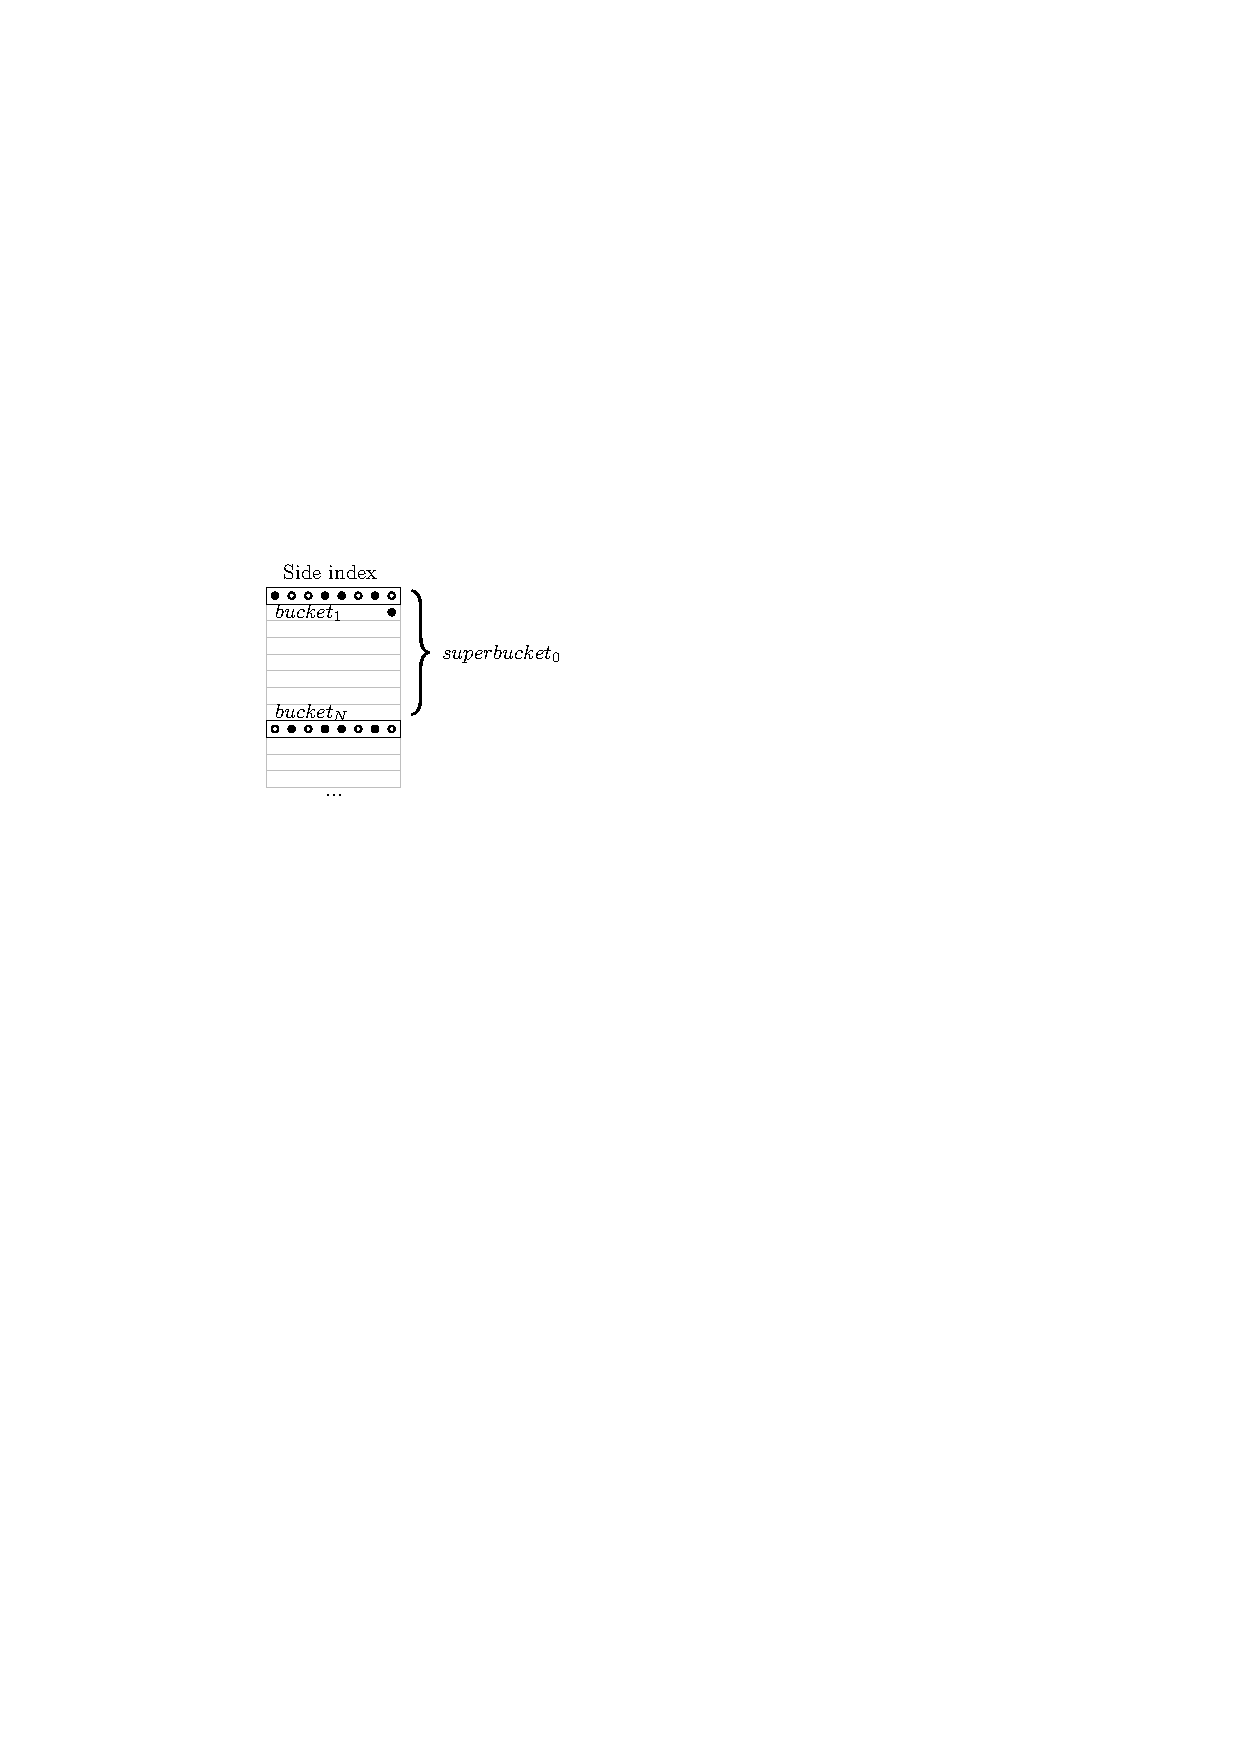
\includegraphics{img/bucketshop.pdf}
	\caption{Bucket and superbuckets in an array}
	\vspace{1cm}
\end{wrapfigure}

The structure is illustrated in Figure \ref{figure-bucketshop} and pseudocode
implementation in Figure \ref{figure-bucketshop-pseudocode}. Memory allocation
is expected to be done automatically in {\tt vector} class and the array should
be resized on first access beyond current boundary.  This allows the structure
to occupy only as much memory as is necessary to store a set of size at most
$\O(\max(E))$.

\begin{figure}[h!]
	\label{figure-bucketshop-pseudocode}
\begin{tcolorbox}
\begin{lstlisting}[language=c++,tabsize=2]
struct superbucket {
	uint64_t bits[];
};

struct universe_index {
	vector<struct superbucket> superbuckets;
};

void universe_index::INSERT(offset, hash, data) {
	superbuckets[offset]->bits[hash].bit[data] = 1;
}

vector<element> universe_index::ENUMERATE(hash) {
	vector<element> candidates;
	for (sb in superbuckets) {
		for (i = 0 .. 63) {
			if (sb->bits[hash].bit[i]) 
				candidates.append(bit);
		}
	}
	return candidates;
}
\end{lstlisting}
\end{tcolorbox}
\caption{Bucket and superbuckets prototype and pseudocode}
\end{figure}



